% 图 74.4 —— 由 `checks/emit_hand.py` 自动拼出（probe 精测 + prims2 图元分解）
%%
% ⚠ 这是**稿子不是成品**：跑 `checks/checkhand.py 74.4` 看指标 + 看叠合图。
%%
%% ⚠ 待核：
%   · 本图 probe 报出阴影族 1 个 —— **本脚本不生成阴影**（要照原书手写）；prims2 的 strokes 里可能含阴影线，核对时留意别画重
%   · 可疑字形 1 项（空心圈 ⊙ 常被认成字母 o）—— 见文件末
%%
\documentclass[12pt]{standalone}
\usepackage{fontspec}
\setsansfont{Arial}
\newfontfamily\mfallback{DejaVu Sans}
\usepackage{tikz}
\begin{document}
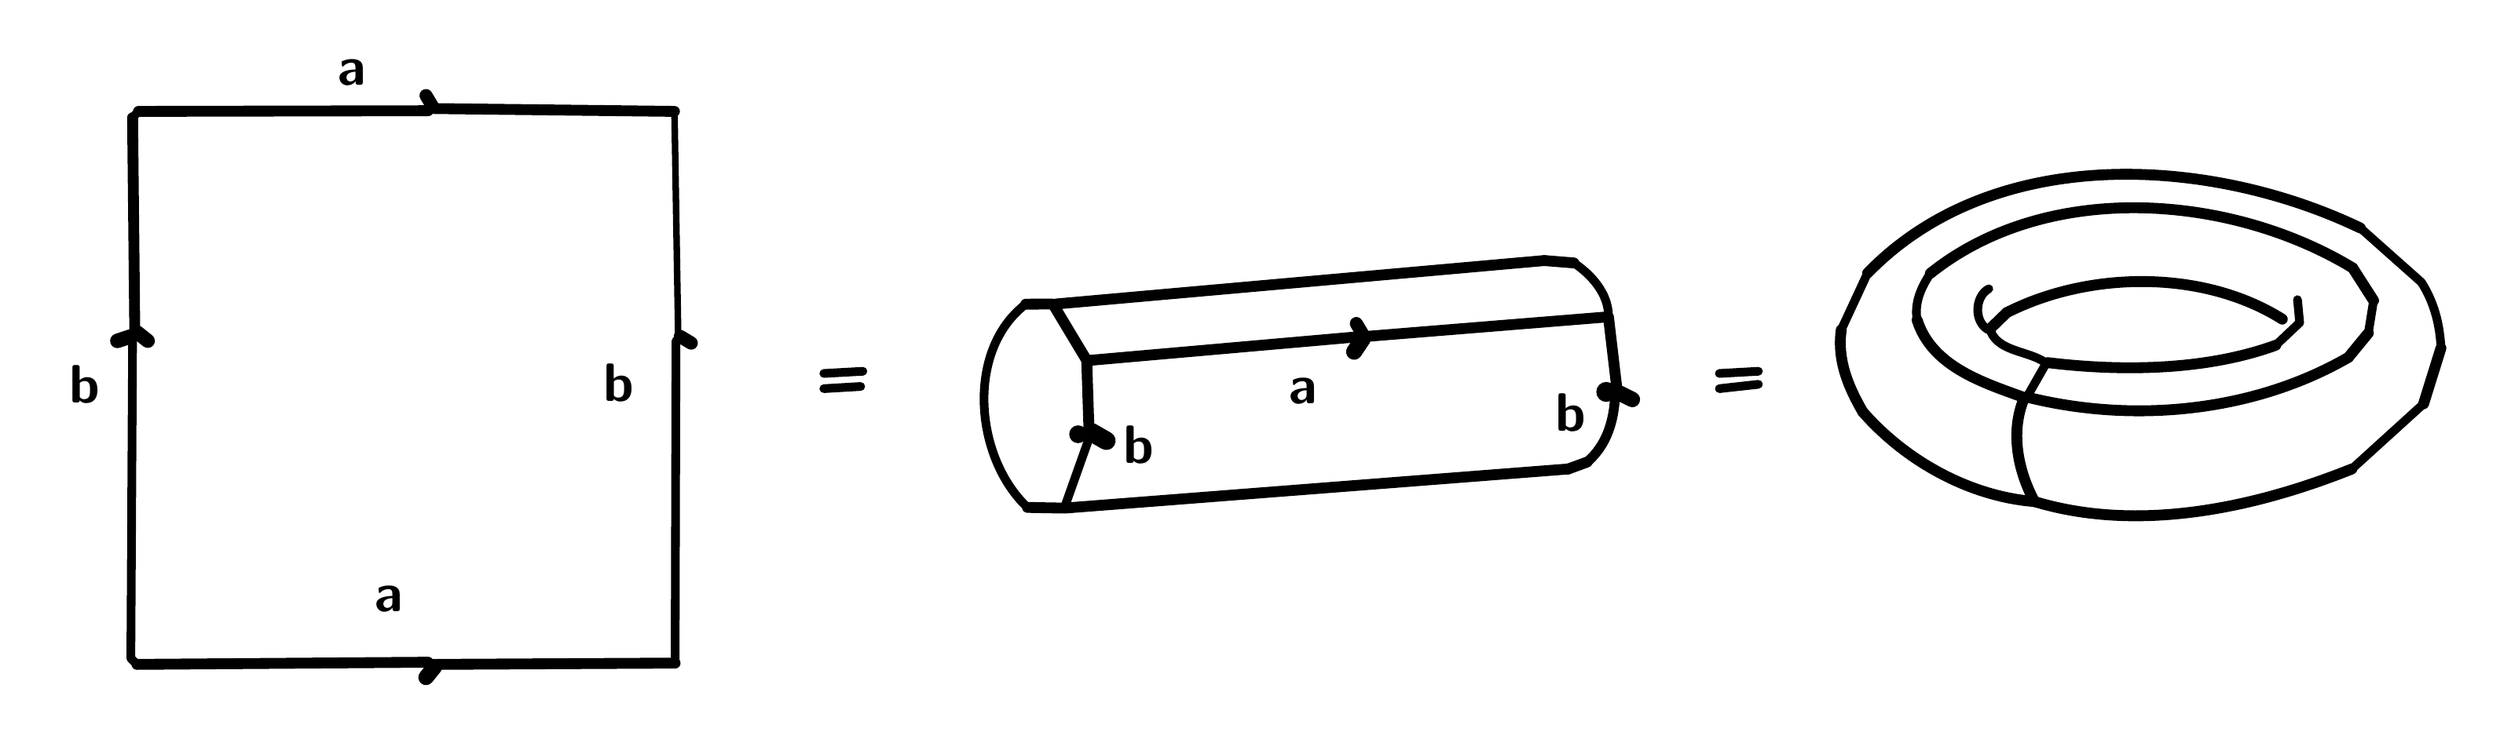
\begin{tikzpicture}[x=1pt, y=-1pt, line width=4.0pt, line cap=round, line join=round]

  %% ════ 填充区（prims2 的 fills）════

  %% ════ 直线段（prims2 的 strokes）════
  \draw[line width=4.0pt] (923.0,172.0) -- (931.0,158.0);
  \draw[line width=5.0pt] (714.1,111.1) -- (700.5,110.0);
  \draw[line width=5.0pt] (700.5,110.0) -- (476.0,130.0);
  \draw[line width=4.0pt] (480.0,223.0) -- (491.0,192.0);
  \draw[line width=7.1pt] (735.0,171.0) -- (741.0,174.0);
  \draw[line width=4.0pt] (369.0,162.0) -- (387.0,161.0);
  \draw[line width=5.0pt] (490.0,156.0) -- (475.0,131.0);
  \draw[line width=6.5pt] (53.0,143.0) -- (58.0,147.0);
  \draw[line width=5.0pt] (618.0,145.0) -- (729.0,136.0);
  \draw[line width=6.0pt] (186.0,34.0) -- (189.0,39.0);
  \draw[line width=5.0pt] (474.0,130.0) -- (461.9,130.1);
  \draw[line width=5.0pt] (462.7,223.7) -- (479.0,224.0);
  \draw[line width=5.0pt] (906.0,141.0) -- (913.2,134.0);
  \draw[line width=4.0pt] (799.0,161.0) -- (781.0,162.0);
  \draw[line width=4.0pt] (1037.0,149.0) -- (1048.0,138.6);
  \draw[line width=4.0pt] (1048.0,138.6) -- (1047.0,128.0);
  \draw[line width=4.0pt] (799.0,167.0) -- (781.0,169.0);
  \draw[line width=4.0pt] (369.0,169.0) -- (386.0,168.0);
  \draw[line width=4.0pt] (301.0,147.0) -- (300.6,295.4);
  \draw[line width=5.0pt] (300.6,295.4) -- (191.0,296.0);
  \draw[line width=5.0pt] (52.0,142.0) -- (51.0,44.2);
  \draw[line width=4.0pt] (51.0,44.2) -- (53.7,41.3);
  \draw[line width=5.0pt] (53.7,41.3) -- (187.0,41.0);
  \draw[line width=6.7pt] (50.0,145.0) -- (44.0,147.0);
  \draw[line width=7.4pt] (613.0,152.0) -- (617.0,146.0);
  \draw[line width=5.0pt] (480.0,224.0) -- (711.5,206.0);
  \draw[line width=5.0pt] (711.5,206.0) -- (720.2,202.8);
  \draw[line width=4.0pt] (51.0,146.0) -- (50.2,293.2);
  \draw[line width=4.0pt] (50.2,293.2) -- (53.0,296.0);
  \draw[line width=5.0pt] (53.0,296.0) -- (187.0,295.0);
  \draw[line width=5.0pt] (491.0,156.0) -- (616.0,145.0);
  \draw[line width=5.0pt] (1072.4,113.4) -- (1082.0,128.4);
  \draw[line width=4.0pt] (1082.0,128.4) -- (1079.6,143.4);
  \draw[line width=5.0pt] (1079.6,143.4) -- (1070.4,154.6);
  \draw[line width=6.0pt] (614.0,139.0) -- (617.0,144.0);
  \draw[line width=3.0pt] (302.0,144.0) -- (300.3,41.3);
  \draw[line width=5.0pt] (300.3,41.3) -- (190.0,40.0);
  \draw[line width=8.5pt] (499.0,193.0) -- (492.0,189.0);
  \draw[line width=7.1pt] (186.0,302.0) -- (190.0,297.0);
  \draw[line width=5.0pt] (730.0,136.0) -- (734.0,170.0);
  \draw[line width=5.0pt] (490.0,157.0) -- (491.0,188.0);
  \draw[line width=6.1pt] (308.0,148.0) -- (303.0,145.0);
  \draw[line width=4.0pt] (837.1,141.9) -- (849.2,115.8);
  \draw[line width=4.0pt] (1075.9,95.0) -- (1104.0,120.0);
  \draw[line width=5.0pt] (1113.0,150.3) -- (1105.0,176.0);
  \draw[line width=4.0pt] (1105.0,176.0) -- (1072.0,206.0);

  %% ════ 曲线（prims2 的 curves —— 三段式，坐标同为 (y,x)）════
  \draw[line width=4.0pt] (730.0,135.0) .. controls (729.7,125.1) and (722.3,116.6) .. (714.1,111.1);
  \draw[line width=4.0pt] (905.0,123.0) .. controls (898.4,126.5) and (898.0,138.6) .. (905.0,142.0);
  \draw[line width=4.0pt] (461.9,130.1) .. controls (434.2,151.3) and (438.3,200.7) .. (462.7,223.7);
  \draw[line width=5.0pt] (913.2,134.0) .. controls (951.2,114.7) and (1003.7,114.1) .. (1040.0,137.0);
  \draw[line width=5.0pt] (921.0,174.0) .. controls (914.8,189.4) and (918.5,207.1) .. (926.0,221.0);
  \draw[line width=5.0pt] (932.0,157.0) .. controls (965.6,161.1) and (1004.7,160.8) .. (1037.0,149.0);
  \draw[line width=4.5pt] (720.2,202.8) .. controls (729.1,195.1) and (732.4,184.2) .. (733.0,173.0);
  \draw[line width=4.0pt] (931.0,157.0) .. controls (923.4,151.6) and (910.1,152.1) .. (906.0,143.0);
  \draw[line width=5.0pt] (921.0,173.0) .. controls (902.7,166.3) and (878.9,159.0) .. (872.0,137.4);
  \draw[line width=4.0pt] (872.0,137.4) .. controls (870.6,129.2) and (874.0,122.2) .. (878.1,115.9);
  \draw[line width=5.0pt] (878.1,115.9) .. controls (931.8,72.9) and (1016.0,79.2) .. (1072.4,113.4);
  \draw[line width=5.0pt] (1070.4,154.6) .. controls (1027.2,179.6) and (972.2,185.2) .. (923.0,173.0);
  \draw[line width=5.0pt] (926.0,221.0) .. controls (897.0,218.7) and (867.5,203.1) .. (847.0,179.7);
  \draw[line width=5.0pt] (847.0,179.7) .. controls (840.5,168.4) and (835.1,156.1) .. (837.1,141.9);
  \draw[line width=5.0pt] (849.2,115.8) .. controls (907.2,55.9) and (1006.7,61.8) .. (1075.9,95.0);
  \draw[line width=4.0pt] (1104.0,120.0) .. controls (1109.8,129.1) and (1112.5,139.3) .. (1113.0,150.3);
  \draw[line width=5.0pt] (1072.0,206.0) .. controls (1027.8,223.7) and (974.3,235.6) .. (926.0,221.0);

  %% ════ 实心点 ════
  \fill (729.0,170.5) circle (4.6);
  \fill (486.0,190.0) circle (4.1);

  %% ════ 标签（probe 直接给的 \node 行）════
  %% ⚠ 全部补了 fill=white：文字在最上层，否则与曲线交叉干扰
     \node[anchor=center,inner sep=0pt,fill=white,font=\fontsize{32.9}{41.1}\selectfont] at (152.1,23.6) {\textsf{\textbf{\textit{a}}}};   % box(143,13,16,18)
     \node[anchor=center,inner sep=0pt,fill=white,font=\fontsize{30.7}{38.3}\selectfont] at (28.8,166.8) {\textsf{\textbf{\textit{b}}}};   % box(19,154,17,23)
     \node[anchor=center,inner sep=0pt,fill=white,font=\fontsize{30.0}{37.5}\selectfont] at (274.8,166.2) {\textsf{\textbf{\textit{b}}}};   % box(265,154,17,22)
     \node[anchor=center,inner sep=0pt,fill=white,font=\fontsize{33.0}{41.2}\selectfont] at (589.6,170.1) {\textsf{\textbf{\textit{a}}}};   % box(580,160,17,17)
     \node[anchor=center,inner sep=0pt,fill=white,font=\fontsize{30.7}{38.3}\selectfont] at (712.8,179.8) {\textsf{\textbf{\textit{b}}}};   % box(703,167,17,23)
     \node[anchor=center,inner sep=0pt,fill=white,font=\fontsize{30.7}{38.3}\selectfont] at (513.8,194.8) {\textsf{\textbf{\textit{b}}}};   % box(504,182,17,23)
     \node[anchor=center,inner sep=0pt,fill=white,font=\fontsize{32.0}{40.0}\selectfont] at (169.1,266.1) {\textsf{\textbf{\textit{a}}}};   % box(160,256,16,17)

  % 钉死画布：否则超出的图元/控制点会把页面撑大，1:1 回比就失准
  \pgfresetboundingbox
  \path[use as bounding box] (0,0) rectangle (1130,317);
\end{tikzpicture}
\end{document}

% ⚠ 待核清单（probe 拿不准，人眼过一遍）：
%   · 未识别/跳过：⑤ 跳过/未识别的字形
